\documentclass[12pt]{article}
\usepackage[utf8]{inputenc}
\usepackage{float}
\usepackage{amsmath}
\usepackage{amssymb}
\usepackage{multicol}
\usepackage[shortlabels]{enumitem}
\usepackage{tikz}
\usepackage{graphicx}
\graphicspath{ {imgs/} }
\usepackage{listings}


\usepackage[hmargin=3cm,vmargin=6.0cm]{geometry}
\topmargin=-2cm
\addtolength{\textheight}{6.5cm}
\addtolength{\textwidth}{2.0cm}
\setlength{\oddsidemargin}{0.0cm}
\setlength{\evensidemargin}{0.0cm}

\begin{document}

\section*{Student Information}
Full Name: Berk Ulutaş \\
Id Number: 2522084 \\

\section*{Answer 1}
\subsection*{a)}
$G_1$ represents a context-free grammar which generates $n$ 0's followed by $n$ 1's $(0^n1^n \text{ where } n \geq 0)$ or $n$ 1's followed by $n$ 0's $(1^n0^n \text{ where } n \geq 0)$.
\subsection*{b)}
Yes, there are 2 distinct parse trees for $e \in L(G_1)$. So, $G_1$ is ambiguous. \\ 

\begin{minipage}{0.4\textwidth}
\begin{tikzpicture}
  \node {$S$}
    child {node {$A$}
        child {node {$e$}}
    };
\end{tikzpicture}
\end{minipage}
\begin{minipage}{0.4\textwidth}
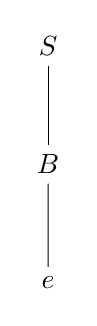
\begin{tikzpicture}
  \node {$S$}
    child {node {$B$}
        child {node {$e$}}
    };
\end{tikzpicture}
\end{minipage}


\section*{Answer 2}
\subsection*{a)}
There are two distinct parse trees for $aa \in L(G_2)$. So, $G_2$ is ambiguous. \\

\begin{minipage}{0.4\textwidth}
\begin{tikzpicture}
  \node {$S$}
    child {node {$A$}
        child {node {$a$}}
        child {node {$A$}
            child {node {$a$}}
            child {node {$A$}
            child {node {$e$}}}}}
    child {node {$B$}
      child {node {$e$}}
    };
\end{tikzpicture}
\end{minipage}
\begin{minipage}{0.4\textwidth}
\begin{tikzpicture}
  \node {$S$}
    child {node {$A$}
        child {node {$a$}}
        child {node {$A$}
            child {node {$a$}}
            }}
    child {node {$B$}
      child {node {$e$}}
    };
\end{tikzpicture}
\end{minipage}

\subsection*{b)}
$G_2 = \{V, \Sigma, R, S\}$ where $V = \{a,b,S,A,B\}$, $\Sigma =  \{a,b\}$ and R: \\
$ S \rightarrow AB$ \\ 
$ A \rightarrow aA | e$ \\ 
$ B \rightarrow bB | e$ 
\subsection*{c)}
$$S \rightarrow AB \rightarrow  aAB \rightarrow aB \rightarrow  abB \rightarrow abbB \rightarrow abbbB \rightarrow abbb$$
\\
\begin{center}
\begin{tikzpicture}
  \node {$S$}
    child {node [xshift = -0.5cm]{$A$}
        child {node {$a$}}
        child {node {$A$}
            child {node {$e$}}
            }}
    child {node [xshift = +0.5cm]{$B$}
      child {node {$b$}}
      child {node {$B$}
        child {node {$b$}}
        child {node {$B$}
            child {node {$b$}}
            child {node {$B$} 
                child {node {$e$}}}
               }}
    };
\end{tikzpicture}
\end{center}

\section*{Answer 3}
\subsection*{a)}
According to our textbook: "we call a language $L \subseteq \Sigma^*$ deterministic context-free if $L\$ = L(M)$ for some deterministic pushdown automaton $M$. Here \$ is a new symbol, not in $\Sigma$, which is appended to each input string for the purpose of marking its end."   (page 159). So, for this question \$ will be represent end of string. 
\subsubsection*{i)}
$$L_1 = \{ca^mb^n | m \neq n\} \cup \{da^mb^{2m} | m \geq 0\}$$
The language is deterministic context-free since it is accepted by the following DPDA.
\begin{itemize}
    \item Start with pushing bottom of stack symbol the stack, and change state to $p$
    \item If machine reads $c$ change state to $q$
    \begin{itemize}
        \item For every $a$ read from input push $a$ to the stack. 
        \item If input completely read (read \$) and stack is not empty then change state to $t$, empty stack and accept.
        \item If stack is empty (top of the stack is $\bot$) and input has not finished then change state to $u$ finish reading input and accept.
        \item If machine read all $a$'s, there is remaining $b$'s and stack is not empty. Read at least one $b$, change state to $r$. For every $b$ read pop $a$ from stack. If input completely read (read \$) and stack is not empty then change state to $t$, empty stack and accept. If stack is empty (top of the stack is $\bot$) and input has not finished then change state to $u$ finish reading input and accept.
    \end{itemize}
    \item If machine reads $d$ change state to $v$
    \begin{itemize}
        \item For every $a$ read, push $aa$ to the stack.
        \item If input empty (read \$) and stack is empty (top of the stack $\bot$) then change state to $f_3$, and accept.
        \item To process $b$'s after reading first $b$ and popping $a$, change state to $w$. For every $b$ read, pop $a$ from the stack. If input completely read (read \$) and stack is empty then change state to $f_3$ and accept.
    \end{itemize}
\end{itemize}

$$M = \{K, \Sigma, \Gamma, s, F, \Delta\}$$
$$K = \{s,p,q,r,t,u,v,w,f_1,f_2,f_3\}$$
$$\Sigma = \{a,b,c,d,\$\}$$
$$\Gamma = \{a, \bot\}$$
$$F = \{f_1, f_2, f_3\}$$
\begin{equation*}
    \begin{split}
        \Delta = \{&((s,e,e),(p,\bot)), ((p,c,e),(q,e)),\\
                   &((p,d,e),(v,e)), ((q,a,e),(q,a)),\\
                   &((q,\$,a),(t,e)), ((t,e,a),(t,e)),\\
                   &((t,e,\bot),(f_1,e)), ((q,b,\bot),(u,e)),\\
                   &((u,b,e),(u,e)), ((u,\$,e),(f_2,e)),\\
                   &((q,b,a),(r,e)), ((r,b,a),(r,e)),\\
                   &((r,\$,a),(t,e)), ((r,b,\bot),(u,e)),\\
                   &((v,a,e),(v,aa)), ((v,\$,\bot),(f_3,e)),\\
                   &((v,b,a),(w,e)), ((w,b,a),(w,e)),\\
                   &((w,\$,\bot),(f_3,e)) 
                    \}
    \end{split}
\end{equation*}

\begin{center}
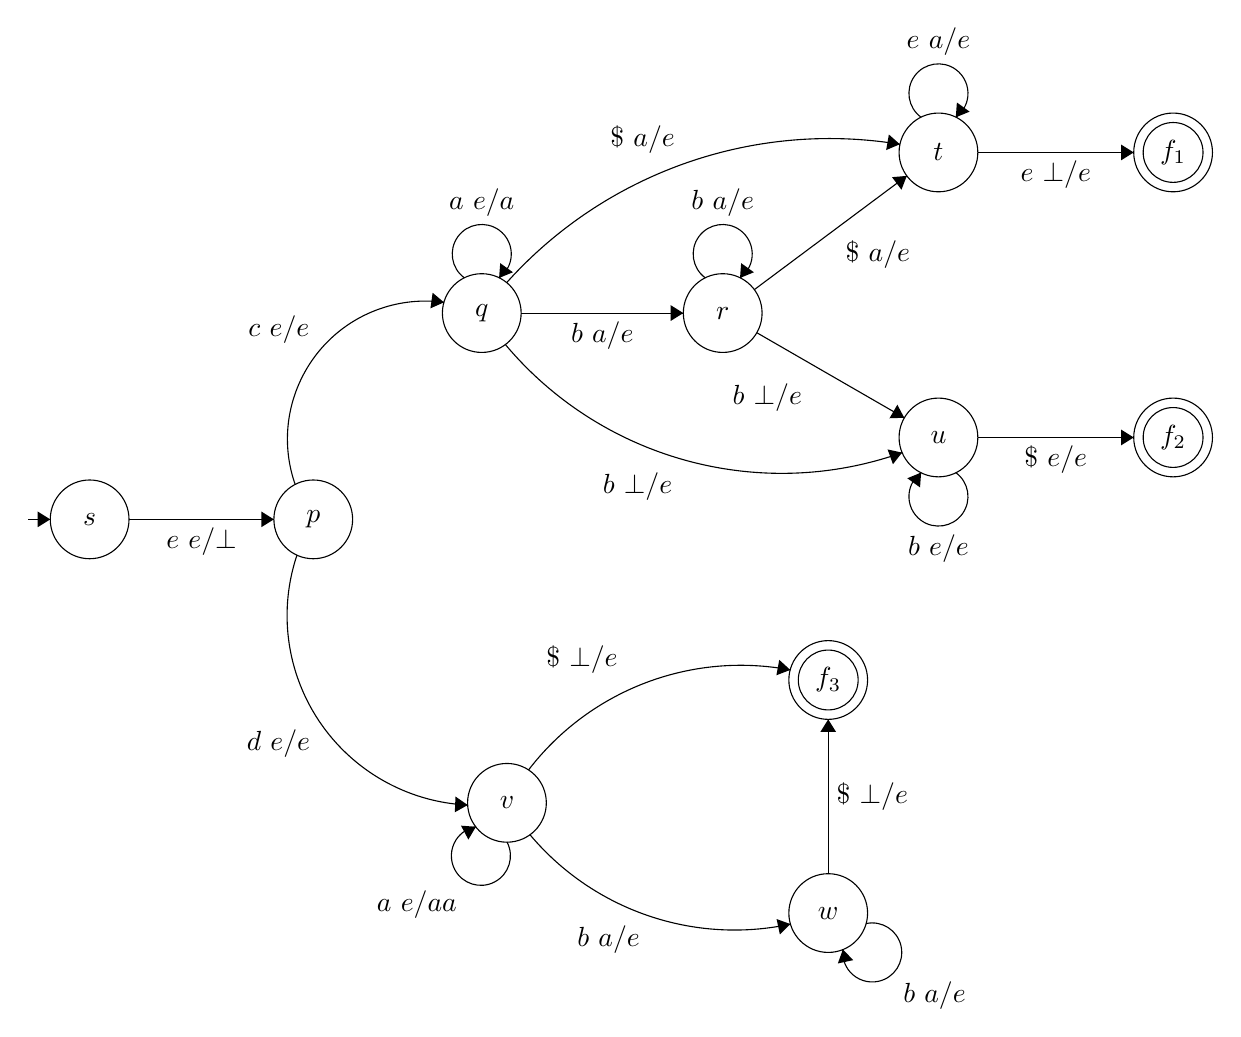
\begin{tikzpicture}[scale=0.2]
\tikzstyle{every node}+=[inner sep=0pt]
\draw [black] (4.1,-28.6) circle (2.5);
\draw (4.1,-28.6) node {$s$};
\draw [black] (18.3,-28.6) circle (2.5);
\draw (18.3,-28.6) node {$p$};
\draw [black] (29,-15.5) circle (2.5);
\draw (29,-15.5) node {$q$};
\draw [black] (44.3,-15.5) circle (2.5);
\draw (44.3,-15.5) node {$r$};
\draw [black] (58,-5.3) circle (2.5);
\draw (58,-5.3) node {$t$};
\draw [black] (72.9,-5.3) circle (2.5);
\draw (72.9,-5.3) node {$f_1$};
\draw [black] (72.9,-5.3) circle (1.9);
\draw [black] (72.9,-23.4) circle (2.5);
\draw (72.9,-23.4) node {$f_2$};
\draw [black] (72.9,-23.4) circle (1.9);
\draw [black] (30.6,-46.6) circle (2.5);
\draw (30.6,-46.6) node {$v$};
\draw [black] (51,-53.6) circle (2.5);
\draw (51,-53.6) node {$w$};
\draw [black] (51,-38.8) circle (2.5);
\draw (51,-38.8) node {$f_3$};
\draw [black] (51,-38.8) circle (1.9);
\draw [black] (58,-23.4) circle (2.5);
\draw (58,-23.4) node {$u$};
\draw [black] (0.2,-28.6) -- (1.6,-28.6);
\fill [black] (1.6,-28.6) -- (0.8,-28.1) -- (0.8,-29.1);
\draw [black] (6.6,-28.6) -- (15.8,-28.6);
\fill [black] (15.8,-28.6) -- (15,-28.1) -- (15,-29.1);
\draw (11.2,-29.1) node [below] {$e\mbox{ }e/\bot$};
\draw [black] (17.152,-26.389) arc (-160.73265:-277.75083:8.761);
\fill [black] (26.6,-14.82) -- (25.88,-14.21) -- (25.74,-15.2);
\draw (18.08,-16.53) node [left] {$c\mbox{ }e/e$};
\draw [black] (28.108,-46.74) arc (-92.72816:-198.57965:12.045);
\fill [black] (28.11,-46.74) -- (27.33,-46.2) -- (27.29,-47.2);
\draw (18.13,-42.85) node [left] {$d\mbox{ }e/e$};
\draw [black] (30.603,-49.09) arc (27.80746:-260.19254:1.875);
\draw (24.88,-52.16) node [below] {$a\mbox{ }e/aa$};
\fill [black] (28.63,-48.12) -- (27.68,-48.05) -- (28.15,-48.93);
\draw [black] (31.97,-44.512) arc (142.51084:79.33816:16.981);
\fill [black] (48.59,-38.16) -- (47.89,-37.52) -- (47.71,-38.5);
\draw (35.36,-38.39) node [above] {$\$\mbox{ }\bot/e$};
\draw [black] (48.603,-54.302) arc (-77.91055:-139.96746:16.963);
\fill [black] (48.6,-54.3) -- (47.72,-53.98) -- (47.93,-54.96);
\draw (37.05,-54.35) node [below] {$b\mbox{ }a/e$};
\draw [black] (53.399,-54.268) arc (102.17983:-185.82017:1.875);
\draw (55.73,-58.81) node [right] {$b\mbox{ }a/e$};
\fill [black] (51.93,-55.91) -- (51.61,-56.8) -- (52.59,-56.59);
\draw [black] (51,-51.1) -- (51,-41.3);
\fill [black] (51,-41.3) -- (50.5,-42.1) -- (51.5,-42.1);
\draw (51.5,-46.2) node [right] {$\$\mbox{ }\bot/e$};
\draw [black] (27.898,-13.267) arc (234:-54:1.875);
\draw (29,-9.38) node [above] {$a\mbox{ }e/a$};
\fill [black] (30.1,-13.27) -- (30.98,-12.91) -- (30.17,-12.33);
\draw [black] (31.5,-15.5) -- (41.8,-15.5);
\fill [black] (41.8,-15.5) -- (41,-15) -- (41,-16);
\draw (36.65,-16) node [below] {$b\mbox{ }a/e$};
\draw [black] (43.198,-13.267) arc (234:-54:1.875);
\draw (44.3,-9.38) node [above] {$b\mbox{ }a/e$};
\fill [black] (45.4,-13.27) -- (46.28,-12.91) -- (45.47,-12.33);
\draw [black] (30.583,-13.566) arc (138.09788:80.65813:27.544);
\fill [black] (55.55,-4.78) -- (54.85,-4.16) -- (54.68,-5.15);
\draw (39.21,-5.39) node [above] {$\$\mbox{ }a/e$};
\draw [black] (56.898,-3.067) arc (234:-54:1.875);
\draw (58,0.83) node [above] {$e\mbox{ }a/e$};
\fill [black] (59.1,-3.07) -- (59.98,-2.71) -- (59.17,-2.13);
\draw [black] (60.5,-5.3) -- (70.4,-5.3);
\fill [black] (70.4,-5.3) -- (69.6,-4.8) -- (69.6,-5.8);
\draw (65.45,-5.8) node [below] {$e\mbox{ }\bot/e$};
\draw [black] (46.31,-14.01) -- (55.99,-6.79);
\fill [black] (55.99,-6.79) -- (55.05,-6.87) -- (55.65,-7.67);
\draw (54.15,-10.9) node [below] {$\$\mbox{ }a/e$};
\draw [black] (46.47,-16.75) -- (55.83,-22.15);
\fill [black] (55.83,-22.15) -- (55.39,-21.32) -- (54.89,-22.18);
\draw (47.13,-19.96) node [below] {$b\mbox{ }\bot/e$};
\draw [black] (55.694,-24.362) arc (-70.48513:-139.99167:22.904);
\fill [black] (55.69,-24.36) -- (54.77,-24.16) -- (55.11,-25.1);
\draw (38.89,-25.62) node [below] {$b\mbox{ }\bot/e$};
\draw [black] (59.102,-25.633) arc (54:-234:1.875);
\draw (58,-29.53) node [below] {$b\mbox{ }e/e$};
\fill [black] (56.9,-25.63) -- (56.02,-25.99) -- (56.83,-26.57);
\draw [black] (60.5,-23.4) -- (70.4,-23.4);
\fill [black] (70.4,-23.4) -- (69.6,-22.9) -- (69.6,-23.9);
\draw (65.45,-23.9) node [below] {$\$\mbox{ }e/e$};
\end{tikzpicture}
\end{center}

\subsubsection*{ii)} $$L_2 = \{a^mcb^n | m \neq n\} \cup \{a^mdb^{2m} | m \geq 0\}$$
The language is deterministic context-free since it is accepted by the following DPDA.
\begin{itemize}
    \item Start with pushing bottom of stack symbol the stack, and change state to $p$
    \item For every $a$ read from input push $aa$ to the stack
    \item After this step if we read $c$ from input, change state to $q$
    % C READ
    \begin{itemize}
        \item For every $b$ read, pop $aa$. 
        \item If input has finished (read \$) and stack not empty, change state to $u$ and empty stack accept the input.
        \item If stack is empty (top of stack $\bot$) and input has not finished, change state to $t$ and finish reading input. When input has finished (read \$) change state to $f_1$ and accept.
    \end{itemize}
    % D READ
    \item If we read $d$ from input, change state to $r$
    \begin{itemize}
        \item For every $b$ read pop $a$. 
        \item When input finished (read \$) and stack is empty (top of stack $\bot$), change state to $f_2$ and accept it. 
    \end{itemize}
\end{itemize}

$$M = \{K, \Sigma, \Gamma, s, F, \Delta\}$$
$$K = \{s,p,q,r,t,u,f_1,f_2\}$$
$$\Sigma = \{a,b,c,d,\$\}$$
$$\Gamma = \{a, \bot\}$$
$$F = \{f_1, f_2\}$$
\begin{equation*}
    \begin{split}
        \Delta = \{&((s,e,e),(p,\bot)), ((p,a,e),(p,aa)),\\
                   &((p,c,e),(q,e)), ((p,d,e),(r,e)),\\
                   &((q,b,aa),(q,e)), ((q,\$,aa),(u,e)),\\
                   &((u,e,aa),(u,e)), ((u,e,\bot),(f_1,e)),\\
                   &((q,b,\bot),(t,e)), ((t,b,e),(t,e)),\\
                   &((t,\$,e),(f_1,e)), ((r,b,a),(r,e)),\\
                   &((r,\$,\bot),(f_3,e))
                    \}
    \end{split}
\end{equation*}

\begin{center}
\begin{tikzpicture}[scale=0.2]
\tikzstyle{every node}+=[inner sep=0pt]
\draw [black] (4.4,-28.8) circle (3);
\draw (4.4,-28.8) node {$s$};
\draw [black] (20.1,-28.8) circle (3);
\draw (20.1,-28.8) node {$p$};
\draw [black] (36.3,-16.2) circle (3);
\draw (36.3,-16.2) node {$q$};
\draw [black] (40.2,-44.1) circle (3);
\draw (40.2,-44.1) node {$r$};
\draw [black] (53.6,-9.8) circle (3);
\draw (53.6,-9.8) node {$u$};
\draw [black] (53.6,-24) circle (3);
\draw (53.6,-24) node {$t$};
\draw [black] (70.4,-16.2) circle (3);
\draw (70.4,-16.2) node {$f_1$};
\draw [black] (70.4,-16.2) circle (2.4);
\draw [black] (69.7,-44.1) circle (3);
\draw (69.7,-44.1) node {$f_2$};
\draw [black] (69.7,-44.1) circle (2.4);
\draw [black] (7.4,-28.8) -- (17.1,-28.8);
\fill [black] (17.1,-28.8) -- (16.3,-28.3) -- (16.3,-29.3);
\draw (12.25,-29.3) node [below] {$e\mbox{ }e/\bot$};
\draw [black] (22.78,-27.477) arc (144:-144:2.25);
\draw (27.35,-28.8) node [right] {$a\mbox{ }e/aa$};
\fill [black] (22.78,-30.12) -- (23.13,-31) -- (23.72,-30.19);
\draw [black] (37.207,-44.238) arc (-92.15474:-162.40161:17.958);
\fill [black] (37.21,-44.24) -- (36.43,-43.71) -- (36.39,-44.71);
\draw (24.27,-41.08) node [below] {$d\mbox{ }e/e$};
\draw [black] (41.523,-46.78) arc (54:-234:2.25);
\draw (40.2,-51.35) node [below] {$b\mbox{ }a/e$};
\fill [black] (38.88,-46.78) -- (38,-47.13) -- (38.81,-47.72);
\draw [black] (43.2,-44.1) -- (66.7,-44.1);
\fill [black] (66.7,-44.1) -- (65.9,-43.6) -- (65.9,-44.6);
\draw (54.95,-44.6) node [below] {$\$\mbox{ }\bot/e$};
\draw [black] (-0.1,-28.8) -- (1.4,-28.8);
\fill [black] (1.4,-28.8) -- (0.6,-28.3) -- (0.6,-29.3);
\draw [black] (21.164,-25.999) arc (154.23787:101.5121:17.344);
\fill [black] (33.32,-16.54) -- (32.44,-16.21) -- (32.64,-17.19);
\draw (23.52,-19.35) node [above] {$c\mbox{ }e/e$};
\draw [black] (33.634,-14.85) arc (270.8699:-17.1301:2.25);
\draw (28.92,-10.3) node [above] {$b\mbox{ }aa/e$};
\fill [black] (35.75,-13.26) -- (36.24,-12.46) -- (35.24,-12.47);
\draw [black] (38.341,-14.006) arc (132.17477:88.42835:17.575);
\fill [black] (50.62,-9.46) -- (49.84,-8.94) -- (49.81,-9.94);
\draw (40.73,-9.96) node [above] {$\$\mbox{ }aa/e$};
\draw [black] (52.277,-7.12) arc (234:-54:2.25);
\draw (53.6,-2.55) node [above] {$e\mbox{ }aa/e$};
\fill [black] (54.92,-7.12) -- (55.8,-6.77) -- (54.99,-6.18);
\draw [black] (50.68,-24.663) arc (-83.4128:-145.12529:13.842);
\fill [black] (50.68,-24.66) -- (49.83,-24.26) -- (49.94,-25.25);
\draw (39.46,-24.07) node [below] {$b\mbox{ }\bot/e$};
\draw [black] (54.923,-26.68) arc (54:-234:2.25);
\draw (53.6,-31.25) node [below] {$b\mbox{ }e/e$};
\fill [black] (52.28,-26.68) -- (51.4,-27.03) -- (52.21,-27.62);
\draw [black] (56.32,-22.74) -- (67.68,-17.46);
\fill [black] (67.68,-17.46) -- (66.74,-17.35) -- (67.16,-18.25);
\draw (64.92,-20.62) node [below] {$\$\mbox{ }e/e$};
\draw [black] (56.4,-10.87) -- (67.6,-15.13);
\fill [black] (67.6,-15.13) -- (67.03,-14.38) -- (66.67,-15.31);
\draw (58.28,-13.59) node [below] {$e\mbox{ }\bot/e$};
\end{tikzpicture}
\end{center}

\subsection*{b)}
\includegraphics[width=\textwidth] {q3b}

\end{document}

